\documentclass{standalone}
\usepackage{tikz}
\usetikzlibrary{patterns, positioning}


\begin{document}
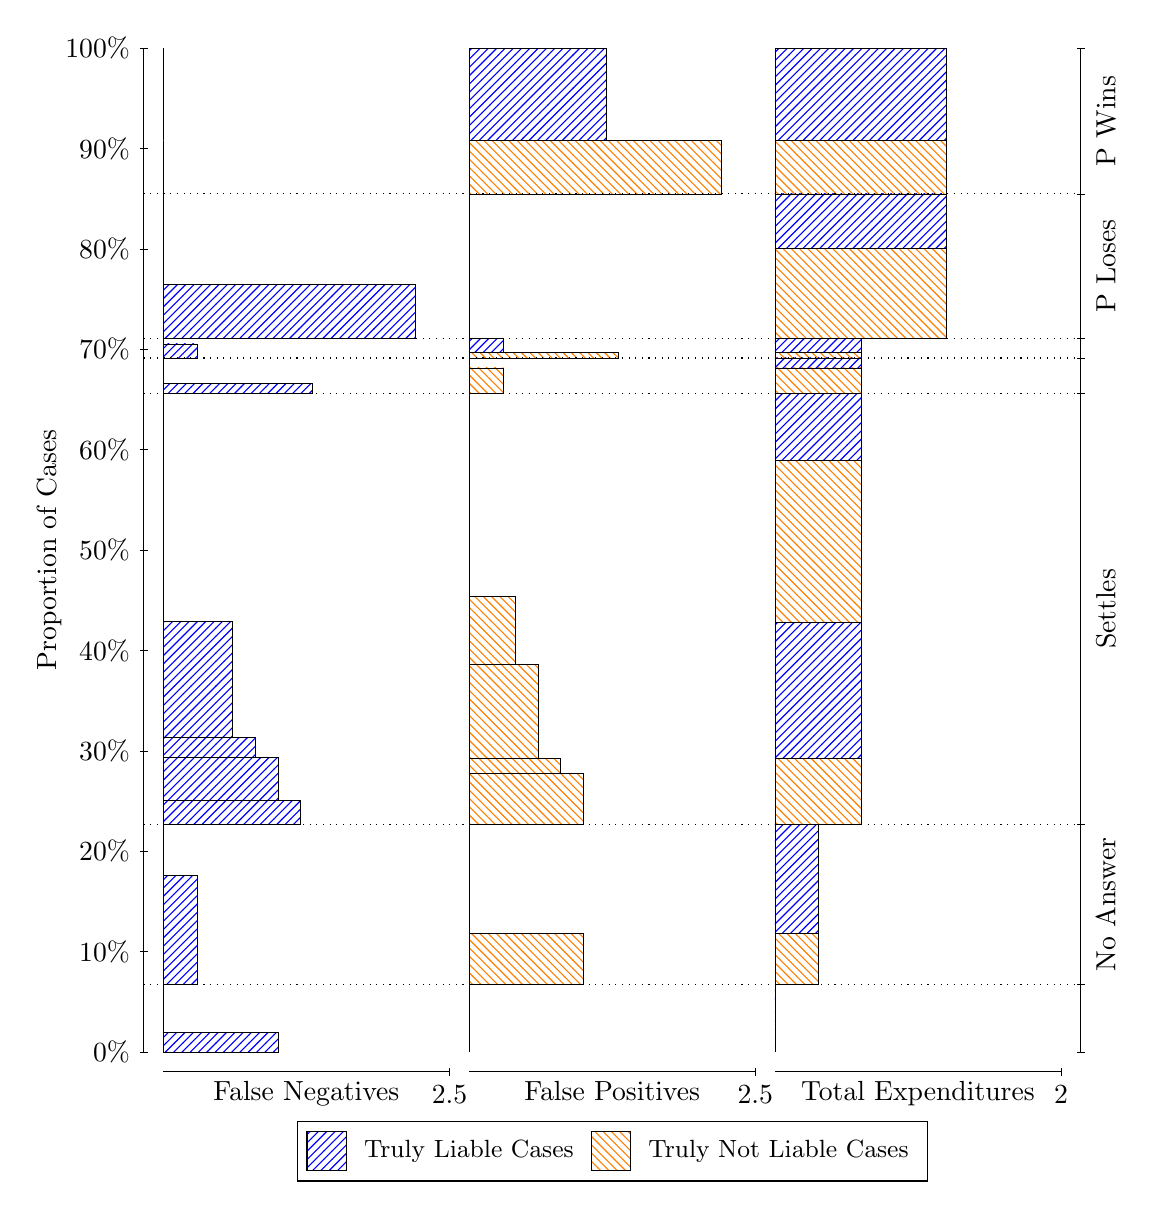
\begin{tikzpicture}
\draw[black, very thin] (1.5,1.75) -- (1.5,14.5);
\node[rotate=90, text=black, anchor=center] at (0.3, 8.125) {Proportion of Cases};
\draw[black, very thin] (1.45,1.75) -- (1.55,1.75);
\node[text=black, anchor=east] at (1.45, 1.75) {0\%};
\draw[black, very thin] (1.45,3.025) -- (1.55,3.025);
\node[text=black, anchor=east] at (1.45, 3.025) {10\%};
\draw[black, very thin] (1.45,4.3) -- (1.55,4.3);
\node[text=black, anchor=east] at (1.45, 4.3) {20\%};
\draw[black, very thin] (1.45,5.575) -- (1.55,5.575);
\node[text=black, anchor=east] at (1.45, 5.575) {30\%};
\draw[black, very thin] (1.45,6.85) -- (1.55,6.85);
\node[text=black, anchor=east] at (1.45, 6.85) {40\%};
\draw[black, very thin] (1.45,8.125) -- (1.55,8.125);
\node[text=black, anchor=east] at (1.45, 8.125) {50\%};
\draw[black, very thin] (1.45,9.4) -- (1.55,9.4);
\node[text=black, anchor=east] at (1.45, 9.4) {60\%};
\draw[black, very thin] (1.45,10.675) -- (1.55,10.675);
\node[text=black, anchor=east] at (1.45, 10.675) {70\%};
\draw[black, very thin] (1.45,11.95) -- (1.55,11.95);
\node[text=black, anchor=east] at (1.45, 11.95) {80\%};
\draw[black, very thin] (1.45,13.225) -- (1.55,13.225);
\node[text=black, anchor=east] at (1.45, 13.225) {90\%};
\draw[black, very thin] (1.45,14.5) -- (1.55,14.5);
\node[text=black, anchor=east] at (1.45, 14.5) {100\%};

\draw[black, very thin] (13.4,1.75) -- (13.4,14.5);
\draw[black, very thin] (13.35,1.75) -- (13.45,1.75);
\node[anchor=west] at (13.35, 1.75) {};
\draw[black, very thin] (13.35,2.6057) -- (13.45,2.6057);
\node[anchor=west] at (13.35, 2.6057) {};
\draw[black, very thin] (13.35,4.6429) -- (13.45,4.6429);
\node[anchor=west] at (13.35, 4.6429) {};
\draw[black, very thin] (13.35,10.113) -- (13.45,10.113);
\node[anchor=west] at (13.35, 10.113) {};
\draw[black, very thin] (13.35,10.564) -- (13.45,10.564);
\node[anchor=west] at (13.35, 10.564) {};
\draw[black, very thin] (13.35,10.814) -- (13.45,10.814);
\node[anchor=west] at (13.35, 10.814) {};
\draw[black, very thin] (13.35,12.648) -- (13.45,12.648);
\node[anchor=west] at (13.35, 12.648) {};
\draw[black, very thin] (13.35,14.5) -- (13.45,14.5);
\node[anchor=west] at (13.35, 14.5) {};

\draw[black, very thin, pattern color=blue, pattern=north east lines] (1.75,1.75) rectangle (3.2033,1.9966);
\draw[black, very thin, pattern color=orange, pattern=north west lines] (1.75,1.9966) rectangle (1.75,2.6057);
\draw[black, very thin, pattern color=blue, pattern=north east lines] (1.75,2.6057) rectangle (2.186,3.9882);
\draw[black, very thin, pattern color=orange, pattern=north west lines] (1.75,3.9882) rectangle (1.75,4.6429);
\draw[black, very thin, pattern color=blue, pattern=north east lines] (1.75,4.6429) rectangle (3.494,4.9474);
\draw[black, very thin, pattern color=blue, pattern=north east lines] (1.75,4.9474) rectangle (3.2033,5.4935);
\draw[black, very thin, pattern color=blue, pattern=north east lines] (1.75,5.4935) rectangle (2.9127,5.7417);
\draw[black, very thin, pattern color=blue, pattern=north east lines] (1.75,5.7417) rectangle (2.622,7.2224);
\draw[black, very thin, pattern color=orange, pattern=north west lines] (1.75,7.2224) rectangle (1.75,10.113);
\draw[black, very thin, pattern color=blue, pattern=north east lines] (1.75,10.113) rectangle (3.6393,10.239);
\draw[black, very thin, pattern color=orange, pattern=north west lines] (1.75,10.239) rectangle (1.75,10.564);
\draw[black, very thin, pattern color=blue, pattern=north east lines] (1.75,10.564) rectangle (2.186,10.744);
\draw[black, very thin, pattern color=orange, pattern=north west lines] (1.75,10.744) rectangle (1.75,10.814);
\draw[black, very thin, pattern color=blue, pattern=north east lines] (1.75,10.814) rectangle (4.9473,11.502);
\draw[black, very thin, pattern color=orange, pattern=north west lines] (1.75,11.502) rectangle (1.75,12.648);
\draw[black, very thin, pattern color=orange, pattern=north west lines] (1.75,12.648) rectangle (1.75,13.327);
\draw[black, very thin, pattern color=blue, pattern=north east lines] (1.75,13.327) rectangle (1.75,14.5);
\draw[black, very thin, pattern color=orange, pattern=north west lines] (5.6333,1.75) rectangle (5.6333,2.3592);
\draw[black, very thin, pattern color=blue, pattern=north east lines] (5.6333,2.3592) rectangle (5.6333,2.6057);
\draw[black, very thin, pattern color=orange, pattern=north west lines] (5.6333,2.6057) rectangle (7.0867,3.2604);
\draw[black, very thin, pattern color=blue, pattern=north east lines] (5.6333,3.2604) rectangle (5.6333,4.6429);
\draw[black, very thin, pattern color=orange, pattern=north west lines] (5.6333,4.6429) rectangle (7.0867,5.2903);
\draw[black, very thin, pattern color=orange, pattern=north west lines] (5.6333,5.2903) rectangle (6.796,5.479);
\draw[black, very thin, pattern color=orange, pattern=north west lines] (5.6333,5.479) rectangle (6.5053,6.6697);
\draw[black, very thin, pattern color=orange, pattern=north west lines] (5.6333,6.6697) rectangle (6.2147,7.5335);
\draw[black, very thin, pattern color=blue, pattern=north east lines] (5.6333,7.5335) rectangle (5.6333,10.113);
\draw[black, very thin, pattern color=orange, pattern=north west lines] (5.6333,10.113) rectangle (6.0693,10.438);
\draw[black, very thin, pattern color=blue, pattern=north east lines] (5.6333,10.438) rectangle (5.6333,10.564);
\draw[black, very thin, pattern color=orange, pattern=north west lines] (5.6333,10.564) rectangle (7.5227,10.634);
\draw[black, very thin, pattern color=blue, pattern=north east lines] (5.6333,10.634) rectangle (6.0693,10.814);
\draw[black, very thin, pattern color=orange, pattern=north west lines] (5.6333,10.814) rectangle (5.6333,11.959);
\draw[black, very thin, pattern color=blue, pattern=north east lines] (5.6333,11.959) rectangle (5.6333,12.648);
\draw[black, very thin, pattern color=orange, pattern=north west lines] (5.6333,12.648) rectangle (8.8307,13.327);
\draw[black, very thin, pattern color=blue, pattern=north east lines] (5.6333,13.327) rectangle (7.3773,14.5);
\draw[black, very thin, pattern color=orange, pattern=north west lines] (9.5167,1.75) rectangle (9.5167,2.3592);
\draw[black, very thin, pattern color=blue, pattern=north east lines] (9.5167,2.3592) rectangle (9.5167,2.6057);
\draw[black, very thin, pattern color=orange, pattern=north west lines] (9.5167,2.6057) rectangle (10.062,3.2604);
\draw[black, very thin, pattern color=blue, pattern=north east lines] (9.5167,3.2604) rectangle (10.062,4.6429);
\draw[black, very thin, pattern color=orange, pattern=north west lines] (9.5167,4.6429) rectangle (10.607,5.479);
\draw[black, very thin, pattern color=blue, pattern=north east lines] (9.5167,5.479) rectangle (10.607,7.2078);
\draw[black, very thin, pattern color=orange, pattern=north west lines] (9.5167,7.2078) rectangle (10.607,9.2623);
\draw[black, very thin, pattern color=blue, pattern=north east lines] (9.5167,9.2623) rectangle (10.607,10.113);
\draw[black, very thin, pattern color=orange, pattern=north west lines] (9.5167,10.113) rectangle (10.607,10.438);
\draw[black, very thin, pattern color=blue, pattern=north east lines] (9.5167,10.438) rectangle (10.607,10.564);
\draw[black, very thin, pattern color=orange, pattern=north west lines] (9.5167,10.564) rectangle (10.607,10.634);
\draw[black, very thin, pattern color=blue, pattern=north east lines] (9.5167,10.634) rectangle (10.607,10.814);
\draw[black, very thin, pattern color=orange, pattern=north west lines] (9.5167,10.814) rectangle (11.697,11.959);
\draw[black, very thin, pattern color=blue, pattern=north east lines] (9.5167,11.959) rectangle (11.697,12.648);
\draw[black, very thin, pattern color=orange, pattern=north west lines] (9.5167,12.648) rectangle (11.697,13.327);
\draw[black, very thin, pattern color=blue, pattern=north east lines] (9.5167,13.327) rectangle (11.697,14.5);
\draw[black, dotted] (1.5,2.6057) -- (13.4,2.6057);
\draw[black, dotted] (1.5,4.6429) -- (13.4,4.6429);
\draw[black, dotted] (1.5,10.113) -- (13.4,10.113);
\draw[black, dotted] (1.5,10.564) -- (13.4,10.564);
\draw[black, dotted] (1.5,10.814) -- (13.4,10.814);
\draw[black, dotted] (1.5,12.648) -- (13.4,12.648);
\draw[black, very thin] (1.75,1.5) -- (5.3833,1.5);
\node[text=black, anchor=north] at (3.5667, 1.5) {False Negatives};
\draw[black, very thin] (5.3833,1.45) -- (5.3833,1.55);
\node[text=black, anchor=north] at (5.3833, 1.45) {2.5};

\draw[black, very thin] (5.6333,1.5) -- (9.2667,1.5);
\node[text=black, anchor=north] at (7.45, 1.5) {False Positives};
\draw[black, very thin] (9.2667,1.45) -- (9.2667,1.55);
\node[text=black, anchor=north] at (9.2667, 1.45) {2.5};

\draw[black, very thin] (9.5167,1.5) -- (13.15,1.5);
\node[text=black, anchor=north] at (11.333, 1.5) {Total Expenditures};
\draw[black, very thin] (13.15,1.45) -- (13.15,1.55);
\node[text=black, anchor=north] at (13.15, 1.45) {2};


\node[text=black, centered, rotate=90] at (13.72, 3.6243) {No Answer};
\node[text=black, centered, rotate=90] at (13.72, 7.3779) {Settles};


\node[text=black, centered, rotate=90] at (13.72, 11.731) {P Loses};
\node[text=black, centered, rotate=90] at (13.72, 13.574) {P Wins};

\draw (7.449999999999999,1.5) node[draw=none] (baseCoordinate) {};
\begin{scope}[align=center]
        \matrix[scale=0.5, draw=black, below=0.5cm of baseCoordinate, nodes={draw}, column sep=0.1cm]{
            \node[rectangle, draw, minimum width=0.5cm, minimum height=0.5cm, pattern color=blue, pattern=north east lines] {}; &
            \node[draw=none, font=\small, text=black] (B) {Truly Liable Cases}; &
            \node[rectangle, draw, minimum width=0.5cm, minimum height=0.5cm, pattern color=orange, pattern=north west lines] {}; &
            \node[draw=none, font=\small, text=black] (B) {Truly Not Liable Cases}; \\
            };
\end{scope}

\end{tikzpicture}
\end{document}